\documentclass[10pt, xcolor=x11names, table]{beamer}
\usetheme{Madrid}
\usecolortheme{dolphin}
\usepackage[latin1]{inputenc}
\usefonttheme{professionalfonts}
\usepackage{times}
\usepackage{tikz}
\usetikzlibrary{decorations.pathreplacing}
\usetikzlibrary{arrows,shapes}
\usetikzlibrary{calc}
\usepackage{animate}
\usepackage{ifthen}
\setbeamertemplate{navigation symbols}{}
\usepackage{amsmath}
\usepackage{verbatim}
\usepackage{units}
\usepackage[absolute,overlay]{textpos}
%\usepackage[texcoord,grid,gridunit=mm,gridcolor=red!10,subgridcolor=green!10]
%{eso-pic}
\usepackage{graphicx}
\newcommand{\putat}[3]{\begin{picture}(0,0)(0,0)\put(#1,#2){#3}\end{picture}}
\usepackage{hyperref}
\usepackage{epstopdf}
\usepackage{accents}
\usepackage{multirow}
\usepackage{xcolor,cancel}
\newcommand\hcancel[2][black]{\setbox0=\hbox{$#2$}%
\rlap{\raisebox{.45\ht0}{\textcolor{#1}{\rule{\wd0}{1pt}}}}#2}
\usepackage{animate}

% Custom numbering using Beamer
\setbeamertemplate{enumerate item}{\arabic{enumi}.}
\setbeamertemplate{enumerate subitem}{\alph{enumii})}
\setbeamertemplate{enumerate subsubitem}{\roman{enumiii}.}

% Custom bullets using Beamer
%\setbeamertemplate{itemize item}{\Large\textbullet}
%\setbeamertemplate{itemize subitem}{\textendash}
%\setbeamertemplate{itemize subsubitem}{\tiny$\blacksquare$}


\title[DSGE]{Dynamic Stochastic General Equilibrium Models of Fluctuations}

\vskip0.1in

\subtitle{\large Session 8: Introduction to DSGE}
%\author[H Hollander]{Hylton Hollander}

\institute[]{ECO5021F: Advanced Macroeconomics\\ University of Cape Town}
\author{}
\date{} % \today


\begin{document}

\AtBeginSection[]
{
\begin{frame}{Table of Contents}
\tableofcontents[currentsection]
\end{frame}
}

\tikzstyle{every picture}+=[remember picture]
\everymath{\displaystyle}

\frame{\titlepage}


\begin{frame}
\frametitle{Readings}
Required
\begin{itemize}
\item \textbf{Chapter 7.1$-$7.4, 7.6$-$7.7}  (\textcolor{blue}{Introduction to DSGE and Calvo pricing})
\item \textbf{Chapter 7.8 to 7.10} (\textcolor{blue}{Canonical DSGE})
\end{itemize}
Recommended
\begin{itemize}
\item Interview with Greg Mankiw (in \textcolor{blue}{Snowdown and Vane})
\end{itemize}
\end{frame}



\begin{frame}
\frametitle{Romer's ``building blocks''}
\begin{itemize}
\item \textbf{Romer} uses a common framework to present different dynamic models with nominal imperfections
\item State vs. time dependent models [\textcolor{blue}{Discuss}]
\item This is a \textbf{discrete time model} %(think Diamond model/ \textcolor{blue}{Lecture 7})
\item Firms are \textbf{imperfectly competitive} (have some market power)
\item Production uses only labour as an input %$\rightarrow$ very simple one-for-one model we used in \textcolor{blue}{Lecture 8}
\begin{align*}
  C_{it} = Y_{it} = L_{it}
\end{align*}
\item Closed economy with no government
\end{itemize}
\end{frame}

\begin{frame}
\frametitle{Romer's ``building blocks''}
\begin{itemize}
\item \textbf{Households}: Maximise utility, take as given the path of real wages (\textcolor{blue}{perfectly competitive}) and the real interest rate \\~\\
\item \textbf{Firms}: Maximise the present value of their profits, subject to some constraint on the ability to set prices \\~\\
\item \textbf{Central Bank}: Set the path for the real interest rate
\end{itemize}
\end{frame}

\begin{frame}
\frametitle{Households}
\begin{itemize}
\item We will combine the two components of the consumption problem from the previous lectures
\item Intertemporal IS curve and labour supply curve % \textbf{Lecture 7}:  \textbf{Lecture 8}: 
\item Demand for individual goods \\~\\ 
\item In aggregate, we assume that,
\begin{align*}
&\sum_{t=0}^{\infty}\beta^{t}\left[U(C_{t}) -  V(L_{t})\right], \quad 0<\beta<1 \\
\text{which gives} \quad &\sum_{t=0}^{\infty}\beta^{t}\left[\frac{C_{t}^{1-\theta}}{1-\theta} -  B\frac{L_{t}^{\gamma}}{\gamma}\right], \quad \gamma>1,\,\theta>0,\, B>0 \\
\text{where} \quad &C = \left[\int^{1}_{0} C_{i}^{\frac{\eta-1}{\eta}}di\right]^{\frac{\eta}{\eta-1}}, \quad \eta>1
\end{align*}
\end{itemize}
\end{frame}

\begin{frame}
\frametitle{Households}
\small
\begin{itemize}
\item As we found in previous lectures, this will yield a
\begin{enumerate}
\item Labour supply curve
\item Intertemporal IS equation
\end{enumerate}
\item In equilibrium, the increase in household income from $dL$ extra labour must equal the disutility of that increase
\begin{align*}
U^{\prime}(C_{t})\frac{W_{t}}{P_{t}} =  V^{\prime}(L_{t}) \\
\frac{W_{t}}{P_{t}} = \frac{BL^{\gamma-1}_{t}}{C_{t}^{-\theta}}
\end{align*}
\item Because $Y_{t} = L_{t} = C_{t}$, we can substitute for $L_{t}$ and $C_{t}$
\begin{align}
\frac{W_{t}}{P_{t}} = {BY_{t}^{\theta + \gamma-1}}
\end{align}
\item For the intertemporal IS equation we have,
\begin{align}
\ln{Y_{t}} = -\frac{1}{\theta}r_{t} -\frac{1}{\theta}\ln{\beta} + {\ln}{Y_{t+1}}
\end{align}
\end{itemize}
\end{frame}

\begin{frame}
\frametitle{Firm: Dynamic price setting}
\begin{itemize}
\item As previously, the demand for each type of good in any period $t$ is given by,
\begin{align*}
Y_{it} = \left(\frac{P_{it}}{P_{t}}\right)^{-\eta}\cdot{Y_{t}}
\end{align*}
\item Real profit is specified as,
\begin{align*}
\frac{R_{it}}{P_{t}} &= \frac{P_{it}}{P_{t}}Y_{it} - \frac{W_{t}}{P_{t}}L_{it} \\
 &= \left(\frac{P_{it}}{P_{t}}\right)^{1-\eta}Y_{t} - \frac{W_{t}}{P_{t}}\left(\frac{P_{it}}{P_{t}}\right)^{-\eta}Y_{t} \\
&=Y_{t}P_{t}^{\eta-1}(P_{it}^{1-\eta} - W_{t}P_{it}^{-\eta})
\end{align*}
\end{itemize}
\end{frame}

\begin{frame}
\frametitle{Firm: Dynamic price setting}
\begin{itemize}
\item This next part is a bit \textcolor{blue}{tricky}, so let us elaborate on the explanation by \textbf{Romer}
\item Consider the problem of a firm setting it's price that may \textbf{remain in place} for a number of periods
\item We can \emph{normalize} the date of the decision to ``period 0''
\item Firm faces the problem of setting a single price to \textbf{maximise profits} over some horizon \\~\\
\item \textbf{Important}: Firm's profit accrues to households $\rightarrow$ values profits according to \textcolor{blue}{utility they provide}
\end{itemize}
\end{frame}

\begin{frame}
\frametitle{Detour: Diamond model}
\begin{itemize}
\item Remember the Euler equation from the \textbf{Diamond model} (p.79), solving for $1+r_{t+1}$
\begin{align*}
1+r_{t+1} = (1+\rho)\frac{C^{\theta}_{2,t+1}}{C^{\theta}_{1,t}} = (1+\rho)\frac{C^{-\theta}_{1,t}}{C^{-\theta}_{2,t+1}} = (1+\rho)\frac{U^{\prime}(C_{1,t})}{U^{\prime}(C_{2,t+1})}
\end{align*}
\item The RHS of the equation $\rightarrow$ definition of the utility function
\item In the \textbf{Diamond model}, individuals only live for \textcolor{blue}{two periods}, so the comparison is $t$ and $t+1$ \\~\\
\item The owners of firms in our Keynesian model are longer lived, so consumption tradeoffs at \textbf{more distant points in time} need to be considered.
\end{itemize}
\end{frame}


\begin{frame}
\frametitle{Firm: Dynamic price setting}
\small
\begin{itemize}
\item If we were to \textcolor{blue}{generalise} the result from the \textbf{Diamond model} to reflect the tradeoff between consumption at time zero and time $t$, we would get,
\begin{align*}
&1+\bar{r}_{t} = \overbrace{\prod_{s=0}^{t}(1+r_{s})}^\text{Cumulative return} = (1+\rho)^{t}\frac{U^{\prime}(C_{0})}{U^{\prime}(C_{t})} \\
\quad &\frac{1}{1+\bar{r}_{t}} =\left[\frac{1}{(1+\rho)}\right]^{t}\frac{U^{\prime}(C_{t})}{U^{\prime}(C_{0})}  = \beta^{t}\frac{U^{\prime}(C_{t})}{U^{\prime}(C_{0})} = \lambda_{t}
\end{align*}
\item \textbf{Romer} defines the $\textstyle \beta^{t}U^{\prime}(C_{t})/{U^{\prime}(C_{0})}$ as the marginal utility of the representative household's consumption in period $t$ relative to period 0
\item $\lambda_{t}$ $\rightarrow$ discount factor that translates period $t$ profits to period 0 units
\item This discount factor $\lambda_{t}$ is defined this way because firms ultimately belong to households
\item Normally, on the \textbf{firm} side, the \textcolor{blue}{real interest rate} is the ``market'' discount factor that governs the transfer of wealth across time
\item \textbf{In equilibrium} $\rightarrow$ market and subjective discount factors should equal
\end{itemize}
\end{frame}



\begin{frame}
\frametitle{Firm: Dynamic price setting}
\begin{itemize}
\item Another \emph{new} component that is introduced is $q_{t}$ $\rightarrow$ probability that a price $P_{i}$ set today (period 0) has not been changed $t$ periods later
\item This probability depends on the firm's future decisions about whether or not to change price
\item We are essentially going to look at several \textbf{alternative models} for $q_{t}$ (could be state or time dependent)
\item For now, it is only going to be a probability \textbf{parameter}, leaving \textcolor{blue}{determination unspecified}
\end{itemize}
\end{frame}

\begin{frame}
\frametitle{Firm: Dynamic price setting}
\begin{itemize}
\item Problem facing the firm is to set it's price to maximise,
\begin{align*}
\max_{P_{i}} \sum^{\infty}_{t=0}\mathbb{E}_{0}\left[q_{t}\lambda_{t}\frac{R_{i}}{P_{t}}\right]
\end{align*}
\item Substituting for the definition of real profit,
\begin{align*}
\max_{P_{i}} \sum^{\infty}_{t=0}\mathbb{E}_{0}\left[q_{t}\lambda_{t}Y_{t}P_{t}^{\eta-1}(P_{i}^{1-\eta} - W_{t}P_{i}^{-\eta})\right]
\end{align*}
\item We will now add some elements to simplify the problem
\end{itemize}
\end{frame}

\begin{frame}
\frametitle{Firm: Dynamic price setting}
\small
\begin{itemize}
\item Recall (previous lecture) that in the perfectly flexible price setting scenario the problem is static (in each period the optimal price only relies on variables from that period)
\item Optimal price $P^{*}_{t}$ is markup over marginal cost,
\begin{align*}
\frac{P^{*}_{t}}{P_{t}} = \frac{\eta}{\eta -1}\frac{W_{t}}{P_{t}} \\
P^{*}_{t} = \frac{\eta}{\eta -1}W_{t} \\
W_{t} = \frac{\eta-1}{\eta}P^{*}_{t}
\end{align*}
\item Substitute this value for $W_{t}$ into the equation from the previous slide,
\begin{align*}
\max_{P_{i}} \sum^{\infty}_{t=0}\mathbb{E}_{0}\left[q_{t}\lambda_{t}Y_{t}P_{t}^{\eta-1}(P_{i}^{1-\eta} - \frac{\eta-1}{\eta}P^{*}_{t}P_{i}^{-\eta})\right]
\end{align*}
\item It is not obvious how we are going to solve this, so we have to make some simplifying assumptions to get to an approximation
\end{itemize}
\end{frame}


\begin{frame}
\frametitle{Approximation of the solution}
\begin{itemize}
\item Two assumptions are made by \textbf{Romer}, to simplify things:
\begin{enumerate}
\item Inflation is low; economy always close to flexible price equilibrium
\item $\beta$ is close to one ($\lambda_{t}$ is close to constant in steady state)
\end{enumerate}
\item First assumption is quite common in complicated non-linear models $\rightarrow$ approximations are often only valid close to the point around the steady state
%\item This type of work will be covered in more detail next year in the \textcolor{blue}{Dynamic Economic Theory} course
\item The first step is going to be to define variables in terms of \textbf{log deviation from steady state}
\item This normalisation means that the log-steady state values are zero, so we only consider the logs of variables
\end{itemize}
\end{frame}

\begin{frame}
\frametitle{Approximation of the solution}
\small
\begin{itemize}
\item Firms problem can be written as,
\begin{align*}
\max_{p_i}\sum^{\infty}_{t=0} \mathbb{E}_{0} \left[q_{t}\lambda_{t}Y_{t}P_{t}^{\eta-1}F(p_{i}, p_{t}^{*})\right]
\end{align*}
\item where $p_{i}$ and $p_{t}^{*}$ denote the logs of $P_{i}$ and $P_{t}^{*}$
\item since we made the assumption that the economy stays near it's flexible price equilibrium,
\begin{enumerate}
  \item eliminate $\lambda_{t}Y_{t}P_{t}^{\eta-1} \rightarrow$ variation negligible relative to variation in $q_{t}$ and $p_{t}^{*}$
  \item $F(p_{i}, p^{*}_{t})$ can be well approximated around the flexible price equilibrium $p_{i} = p_{t}^{*}$
\end{enumerate}
\item Period $t$ profits are maximised where $p_{i} = p_{t}^{*}$
\end{itemize}
\end{frame}

\begin{frame}
\frametitle{Approximation of the solution}
\small
\begin{itemize}
\item Using Taylor expansion, we can write:
\begin{align*}
F(p_{i}, p_{t}^{*}) \approx F(p_{t}^{*}, p_{t}^{*}) + \frac{{\partial}F(p_{i}, p_{t}^{*})}{\partial{p_{i}}}(p_{i} - p_{t}^{*}) + \frac{1}{2}\frac{{\partial^{2}}F(p_{i}, p_{t}^{*})}{\partial^{2}{p_{i}}}(p_{i} - p_{t}^{*})^{2}
\end{align*}
\item We know that $\textstyle \frac{{\partial}F(p_{i}, p_{t}^{*})}{\partial{p_{i}}} = 0$ and  $\textstyle \frac{{\partial^{2}}F(p_{i}, p_{t}^{*})}{\partial^{2}{p_{i}}} < 0 \rightarrow$ profits are maximised
\item Taking this into account we can write the approximation as,
\begin{align*}
F(p_{i}, p_{t}^{*}) \approx F(p_{t}^{*}, p_{t}^{*}) - K(p_{i} - p_{t}^{*})^{2}, \quad K>0
\end{align*}
\item In order to maximise profits, we need to minimize,
\begin{align*}
\min_{p_{i}} \sum_{t=0}^{\infty}q_{t}(p_{i} - p_{t}^{*})^{2}
\end{align*}
\item We drop the expectations operator $\mathbb{E}_{0}$ for now $\rightarrow$ add it back later
\end{itemize}
\end{frame}

\begin{frame}
\frametitle{Approximation of the solution}
\small
\begin{itemize}
\item Minimisation problem is now straightforward,
\begin{align*}
A = &\min_{p_{i}} \sum_{t=0}^{\infty}\left[q_{t}(p_{i} - p_{t}^{*})^{2}\right] \\
 = &\min_{p_{i}} \sum_{t=0}^{\infty}\left[q_{t}(p_{i}^{2} - 2{p_{i}}p_{t}^{*} + p_{t}^{*^2})\right] \\
 = &\min_{p_{i}} \left[\sum_{t=0}^{\infty}q_{t}p_{i}^{2} - 2\sum_{t=0}^{\infty}q_{t}{p_{i}}p_{t}^{*} + \sum_{t=0}^{\infty}q_{t}p_{t}^{*^2}\right] \\
 = &\min_{p_{i}} \left[p_{i}^{2}\sum_{t=0}^{\infty}q_{t} - 2{p_{i}}\sum_{t=0}^{\infty}q_{t}p_{t}^{*} + \sum_{t=0}^{\infty}q_{t}p_{t}^{*^2}\right] \\~\\
\left(\frac{\partial{A}}{\partial{p_{i}}}\right) \qquad &2p_{i}\sum_{t=0}^{\infty}q_{t} = 2\sum_{t=0}^{\infty}q_{t}p_{t}^{*} \\
&p_{i} = \sum_{t=0}^{\infty}\omega_{t}p^{*}_{t}
\end{align*}
\end{itemize}
\end{frame}


\begin{frame}
\frametitle{Firm: Dynamic price setting}
\begin{align*}
p_{i} = \sum_{t=0}^{\infty}\omega_{t}p^{*}_{t}
\end{align*}
\begin{itemize}
\item where $\textstyle \omega_{t} \equiv q_{t}/\sum_{\tau=0}^{\infty}q_{\tau}$
\item Important to know what $p_{i}$ and $p^{*}_{t}$ represent
\begin{itemize}
  \item $p_{i}$ is the \textbf{price that the firm sets in period 0} (knowing it will be in place now, and probably some future period)
  \item $p_{t}^{*}$ is the price that would be ideal for firm to set in period $t$ if it were to set prices independently each period
\end{itemize}
\item Firms would set $p_{i} = p^{*}_{t}$ in every period if there is \textcolor{blue}{no cost of price adjustment}
\item The firm should set a price equal to a \textbf{weighted average} of the ideal prices in each future period
\item It is weighted proportional to the probability that the current (period 0) price will still be in effect during that future period
\end{itemize}
\end{frame}

\begin{frame}
\frametitle{Firm: Dynamic price setting}
\begin{align*}
p_{i} = \sum_{t=0}^{\infty}\omega_{t}p^{*}_{t}
\end{align*}
\begin{itemize}
\item Let us use an \textbf{example} to illustrate how this works
\item Suppose \textbf{it is known} that the newly set price will be in effect for two periods $\rightarrow $ \textcolor{blue}{optimal price} for the firm to set is (\textbf{unweighted}) average between the desired price in the first period and the desired price in the second period
\item If the new price will be in effect for the first period and there is a $50\%$ chance it will be in effect the second period (\textcolor{blue}{but not any longer}) $\rightarrow$ firm sets price at \textbf{weighted average} of the two ideal prices, with 2/3 weight to the first period and 1/3 weight to the second
\end{itemize}
\end{frame}

\begin{frame}
\frametitle{Firm: Dynamic price setting}
\begin{itemize}
\item Finally, in the case of uncertainty, we will reintroduce out expectations operator $\mathbb{E}_{0}$,
\begin{align*}
p_{i} = \sum_{t=0}^{\infty}\omega_{t}\mathbb{E}({p^{*}_{t}})
\end{align*}
\item Finally, let us combine some of our equations (in logarithms) and input them into this function
\begin{align*}
&w_{t}  = p_{t} + b + (\theta+\gamma-1)y_{t}  \\
&p_{t}^{*} = \ln(\frac{\eta}{\eta-1}) + w_{t}  \\
&y_{t} = m_{t} - p_{t}                         \\
\therefore \quad &p_{t}^{*} = \ln(\frac{\eta}{\eta-1}) + p_{t} + b + (\theta+\gamma-1)(m_{t} - p_{t}) \\
&p_{t}^{*} = \phi{m_{t}} + (1-\phi)p_{t} \\
\therefore \quad &p_{i} = \sum_{t=0}^{\infty}\omega_{t}\mathbb{E}[\phi{m_{t}} + (1-\phi)p_{t}]
\end{align*}
\item We have assumed that $\textstyle \ln(\frac{\eta}{\eta-1}) + b = 0$ and $\textstyle \phi = (\theta + \gamma - 1) >0$
\end{itemize}
\end{frame}


\begin{frame}
\frametitle{Predetermined prices: Fischer model}
\begin{itemize}
\item Prices are set in an \textbf{asynchronous} way for two periods
\item \textcolor{blue}{One half of prices} are set by ``\textbf{Group A}'', who presets its price at the end of period $t-1$ for period $t$ and $t+1$
\item This means that A's prices are fixed for two periods
\item ``\textbf{Group B}'' presets at the end of period $t-2$ its price for $t-1$ and $t$
\item In any period, half of prices are ones set in the previous period ($p_{t}^{1}$), and half are set two periods ago ($p_{t}^{2}$), average price is then,
\begin{align*}
p_{t} = \frac{1}{2}(p_{t}^{1} + p_{t}^{2})
\end{align*}
\item Our assumptions imply that $p^{1}_{t}$ equals the expectation as of period $t-1$ of $p_{it}^{*}$ and $p^{2}_{t}$ equals the expectation as of period $t-2$ of $p_{it}^{*}$:
\begin{align*}
&p_{t}^{1} = \mathbb{E}_{t-1}[\phi{m_{t}} + (1-\phi)p_{t}] = \phi\mathbb{E}_{t-1}{m_{t}} + (1-\phi)\frac{1}{2}(p_{t}^{1} + p_{t}^{2}) \\
&p_{t}^{2} = \mathbb{E}_{t-2}[\phi{m_{t}} + (1-\phi)p_{t}] = \phi\mathbb{E}_{t-2}{m_{t}} + (1-\phi)\frac{1}{2}(\mathbb{E}_{t-2}p_{t}^{1} + p_{t}^{2})
\end{align*}
\end{itemize}
\end{frame}

\begin{frame}
\frametitle{Predetermined prices: Fischer model}
\begin{itemize}
\item \textbf{Goal:} Find out how price level and output evolve over time, given the behaviour of $m$
\item Begin by solving for $p^{1}_{t}$, which yields,
\begin{align*}
p_{t}^{1} = \frac{2\phi}{1+\phi}\mathbb{E}_{t-1}{m_{t}} + \frac{1-\phi}{1+\phi}p_{t}^{2}
\end{align*}
\item Take expectation as of $t-2$ on both sides (law of iterated projections),
\begin{align*}
\mathbb{E}_{t-2}\,p_{t}^{1} = \frac{2\phi}{1+\phi}\mathbb{E}_{t-2}{m_{t}} + \frac{1-\phi}{1+\phi}p_{t}^{2}
\end{align*}
\item Now we can substitute this into the equation for $p_{t}^{2}$, which gives us,
\begin{align*}
p_{t}^{2} = \phi\mathbb{E}_{t-2}{m_{t}} + (1-\phi)\frac{1}{2}\left(\frac{2\phi}{1+\phi}\mathbb{E}_{t-2}{m_{t}} + \frac{1-\phi}{1+\phi}p_{t}^{2} + p_{t}^{2}\right)
\end{align*}
\item Solving this expression then gives us,
\begin{align*}
p_{t}^{2} = \mathbb{E}_{t-2}m_{t}
\end{align*}
\end{itemize}
\end{frame}


\begin{frame}
\frametitle{Predetermined prices: Fischer model}
\begin{itemize}
\item Substitute this value for $p_{t}^{2}$ into the equation for $p_{t}^{1}$ and simplify to get,
\begin{align*}
p_{t}^{1} &= \mathbb{E}_{t-2}m_{t} + \frac{2\phi}{1+\phi}\left(\mathbb{E}_{t-1}m_{t} - \mathbb{E}_{t-2}m_{t}\right)
\end{align*}
\item Now substitute into $\textstyle p_{t} = (p_{t}^{1} + p_{t}^{2})/2$ and $y_{t} = m_{t} - p_{t}$, to get:
\begin{align*}
&p_{t} = \mathbb{E}_{t-2}m_{t} + \frac{\phi}{1+\phi}\left(\mathbb{E}_{t-1}m_{t} - \mathbb{E}_{t-2}m_{t}\right) \\
&y_{t} = \frac{1}{1+\phi}\left(\mathbb{E}_{t-1}m_{t} - \mathbb{E}_{t-2}m_{t}\right) + (m_{t} - \mathbb{E}_{t-1}m_{t})
\end{align*}
\item There are a few lessons to be learned from these equations
\begin{enumerate}
  \item \textbf{Unanticipated AD shifts} have real effects ($m_{t} - \mathbb{E}_{t-1}m_{t}$) $\rightarrow$ price setters don't know $m_{t}$ when they set prices
  \item AD shifts that become \textbf{anticipated after the first prices are set} affect output $\rightarrow$ proportion of information about $m_{t}$ that arrives between $t-2$ and $t-1$ is passed into output, the rest into prices
  \item Output does not depend on $\mathbb{E}_{t-2}m_{t}$ $\rightarrow$ once all price setters have had chance to respond, \textbf{demand shocks no longer affect output}
\end{enumerate}
\end{itemize}
\end{frame}

\begin{frame}
\frametitle{Predetermined prices: Fischer model}
\begin{itemize}
\item Some information about the \textbf{real rigidity} parameter $\phi$
\item $\phi$ $\rightarrow$ measures responsiveness of desired real prices to changes in aggregate real output
\item When $\phi$ is small $\rightarrow$ \textcolor{blue}{greater real rigidity}
\begin{itemize}
  \item Large real rigidity means price-setters are reluctant to allow variations in their relative prices (\textbf{prices sticky})
  \item \textbf{Real effects} from money shocks can be large \\~\\
\end{itemize}
\item When $\phi>1$ price-setters are willing to make large price changes
\begin{itemize}
  \item \textbf{Real effects} from money shocks are small
\end{itemize}
\end{itemize}
\end{frame}

\begin{frame}
\frametitle{Calvo model and NK Phillips Curve}
\begin{itemize}
\item Most influential of the staggered price setting models
\item Each period a firm has probability $\alpha$ of getting to change it's price (follows a \emph{\textcolor{blue}{Poisson process}})
\begin{itemize}
\item Implication is that probability that a firm has to change it's price is \textbf{the same each period} (regardless of what happened before)
\end{itemize}
\item The probability of having price fixed until time $j$ is $q_{j} = (1-\alpha)^{j} \rightarrow$ since $(1-\alpha)$ share of the population do not adjust for $j$ periods in a row
\item \textbf{Important} for the result are the following conditions:
\begin{itemize}
  \item Number of firms is large, so by the \textcolor{blue}{law of large numbers} $\rightarrow$ each period exactly a fraction $\alpha$ of firms set their
  prices anew
  \item Firms are chosen at \textbf{random}
\end{itemize}
\end{itemize}
\end{frame}

\begin{frame}
\frametitle{Calvo model and NK Phillips Curve}
\begin{itemize}
\item Average price in any period $t$ is:
\begin{align*}
p_{t} = \alpha{x_{t}} + (1-\alpha)p_{t-1}
\end{align*}
\item where $p$ is the average price and $x$ is the price set by firms who can change their price
\item Average price charged by firms that do not change their levels \textbf{equals} average price charged by all firms in the previous period
\item Subtract $p_{t-1}$ from both sides $\rightarrow$ gives an expression for \textbf{inflation}
\begin{align*}
  p_{t} - p_{t-1} = \pi_{t} = \alpha(x_{t} - p_{t-1})
\end{align*}
\item In what follows we will look for a value of $x_{t} \rightarrow$ average price set by those who can set price (\textbf{reset price})
\end{itemize}
\end{frame}

\begin{frame}
\frametitle{Calvo model and NK Phillips Curve}
\begin{itemize}
\item We begin by looking at the expression for the rule we derived before,
\begin{align*}
p_{i} = \sum_{t=0}^{\infty}\frac{q_{t}}{\textstyle \sum_{\tau =0}^{\infty}q_{\tau}}p^{*}_{t}
\end{align*}
\item One of the assumptions made before was that $\beta \approx 1$ $\rightarrow$ introduce $\beta$ and minimise the firm's loss function to get,
\begin{align*}
  x_{t} = \sum_{j=0}^{\infty}\frac{\beta^{j}q_{j}}{\textstyle \sum_{k=0}^{\infty}\beta^{k}q_{k}}\mathbb{E}_{t}p^{*}_{t+j}
\end{align*}
\item $q_{j} \rightarrow$ probability that the price will still be in effect in period $t+j$
\item ${\textstyle \sum_{k=0}^{\infty}\beta^{k}q_{k}} \rightarrow$ expected number of periods that price will still be in effect
\item \textbf{Poisson} assumption from Calvo implies that $q_{j} = (1-\alpha)^{j}$
\item Using the \textcolor{blue}{geometric sum formula} we get,
\begin{align*}
\sum_{k=0}^{\infty}\beta^{k}q_{k} =  \sum_{k=0}^{\infty}\left[\beta(1-\alpha)\right]^{k} = \frac{1}{1-\beta(1-\alpha)}
\end{align*}
\end{itemize}
\end{frame}

\begin{frame}
\frametitle{Calvo model and NK Phillips Curve}
\small
\begin{itemize}
\item This simplification helps us to rewrite the equation as,
\begin{align*}
  x_{t} = [1-\beta(1-\alpha)]\sum_{j=0}^{\infty}\beta^{j}(1-\alpha)^{j}\mathbb{E}_{t}p^{*}_{t+j}
\end{align*}
\item This equation states that the optimal solution is for the firm to set its price equal to a weighted average of prices it would have expected to set in future (if there were \textbf{no price rigidities})
\item Firm is not able to change price each period $\rightarrow$ tries to keep close to \textbf{optimal frictionless price}
\item Through some further manipulation and the use of $\pi_{t} = \alpha(x_{t} - p_{t-1})$ we will find the \textbf{NK Phillips curve}
\item \textbf{Important:} $x_{t}$ is not the general price level, it is the price that each individual firm sets $\rightarrow$ that is why we need to use our equation for the general price level $p_{t} = \alpha{x_{t}} + (1-\alpha)p_{t-1}$
\end{itemize}
\end{frame}


\begin{frame}
\frametitle{Calvo model and NK Phillips Curve}
\begin{align}
x_{t} &= [1-\beta(1-\alpha)]\sum_{j=0}^{\infty}\beta^{j}(1-\alpha)^{j}\mathbb{E}_{t}p^{*}_{t+j} \\
x_{t} &= [1-\beta(1-\alpha)]\beta(1-\alpha)\mathbb{E}_{t}p^{*}_{t} + \nonumber\\ &\beta(1-\alpha)[1-\beta(1-\alpha)]\left[\sum_{j=0}^{\infty}\beta^{j}(1-\alpha)^{j}\mathbb{E}_{t}p^{*}_{t+1+j}\right] \\
x_{t} &= [1-\beta(1-\alpha)]p^{*}_{t} + \beta(1-\alpha)\mathbb{E}_{t}x_{t+1}
\end{align}
\begin{itemize}
  \item Last equation uses the fact that $p_{t}^{*}$ is known at time $t$ and shifts forward equation (3) one period to get $x_{t+1}$
  \item Subtract $x_{t} - p_{t}$ from both sides gives us,
\end{itemize}
\begin{align*}
(x_{t} - p_{t-1}) - &(p_{t} - p_{t-1}) =  \\
&[1-\beta(1-\alpha)](p^{*}_{t} - p_{t}) + \beta(1-\alpha)(\mathbb{E}_{t}x_{t+1} - p_{t})
\end{align*}
\end{frame}

\begin{frame}
\frametitle{Calvo model and NK Phillips Curve}
\begin{align*}
(x_{t} - p_{t-1}) - &(p_{t} - p_{t-1}) =  \\
&[1-\beta(1-\alpha)](p^{*}_{t} - p_{t}) + \beta(1-\alpha)(\mathbb{E}_{t}x_{t+1} - p_{t})
\end{align*}
\begin{itemize}
  \item From our aggregate price equation, we have that $\textstyle x_{t} - p_{t-1} = {\pi_{t}}/{\alpha}$ and $\mathbb{E}_{t}x_{t+1} - p_{t} = E_{t}\pi_{t+1}/\alpha$.
  \item In addition, $p_{t} - p_{t-1} = \pi_{t}$ and $p_{t}^{*} - p_{t} = \phi{y_{t}}$ (from \textcolor{blue}{Ch. 6, p. 273, (6.60)})
  \item Substituting these values into the equation above gives us the \textbf{NK Phillips curve},
\end{itemize}
\begin{align*}
({\pi_{t}}/{\alpha}) - (\pi_{t}) &= [1-\beta(1-\alpha)]\phi{y_{t}} + \beta(1-\alpha)(E_{t}\pi_{t+1}/\alpha) \\
\pi_{t} &= \frac{\alpha}{1-\alpha}[1-\beta(1-\alpha)]\phi{y_{t}} + \beta\mathbb{E}_{t}\pi_{t+1} \\~\\
\pi_{t}=&\kappa{y_{t}} + \beta\mathbb{E}_{t}\pi_{t+1}, \qquad \kappa \equiv \frac{\alpha[1-(1-\alpha)\beta]\phi}{1-\alpha}
\end{align*}
\end{frame}

\begin{frame}
\frametitle{Example: 3-Equation New Keynesian DSGE model}
\begin{itemize}
\item The basic New Keynesian model with Calvo price setting simplifies to a system of three equations
\begin{enumerate}
\item \textbf{New Keynesian Phillips curve} $\rightarrow$ relating inflation to output gap (\textcolor{blue}{supply side})
\item \textbf{Dynamic IS equation} $\rightarrow$ linking evolution of AD (and the output gap) to the nominal interest rate (\textcolor{blue}{demand side})
\item \textbf{Monetary policy rule} $\rightarrow$ rule for setting the nominal interest rate (normally a Taylor rule)\\~\\
\end{enumerate}
\item Represented below is the system of equations,
\begin{align*}
\pi_{t} &= \kappa{y_{t}} + \beta{\mathbb{E}_{t}}\pi_{t+1} + u_{t}^{s} \,\,\quad\qquad\qquad\qquad \text{NK Phillips curve}\\
y_{t} &= -\frac{1}{\theta}(i_{t} - \mathbb{E}_{t}\pi_{t+1}) + \mathbb{E}_{t}y_{t+1} + u_{t}^{d} \qquad \text{Dynamic IS equation}\\
i_{t} &= \phi_{y}y_{t} + \phi_{\pi}\pi_{t} + u_{t}^{m} \quad\quad\qquad\qquad\qquad \text{Monetary policy rule}
\end{align*}
\end{itemize}
\end{frame}



\begin{frame}
\frametitle{Inflation inertia}
\begin{align*}
\mathbb{E}_{t}\pi_{t+1} - \pi_{t} = \underbrace{\frac{1-\beta}{\beta}}_\text{small$\approx$0.01} \pi_{t} - \frac{\kappa}{\beta}\underbrace{(y_{t} - \bar{y}_{t})}_\text{$\approx$ real MC}
\end{align*}
\begin{itemize}
  \item There are some criticisms of this version of the Phillips curve, \textbf{in the model} we have that
  \begin{itemize}
\item Disinflation can be achieved \textbf{costlessly} (anti-inertia)
\begin{itemize}
\item Inflation inertia $\rightarrow$ inflation is costly to reduce (difficult to do quickly)
\item No tradeoff between inflation and output gap stabilisation
\end{itemize}
\item Anticipated disinflation could \textbf{generate a boom}!
\item Inflation is purely \textcolor{blue}{forward looking} $\rightarrow$ past inflation is irrelevant
\item Inflation leads the output gap measure
\end{itemize}
\item \textbf{Mankiw} (2001) states that the NKPC \emph{cannot even come close to explaining the dynamic effect of monetary policy on inflation and unemployment}
\end{itemize}
\end{frame}


\begin{frame}
\frametitle{Inflation leading the output gap?}
\begin{figure}
\centering
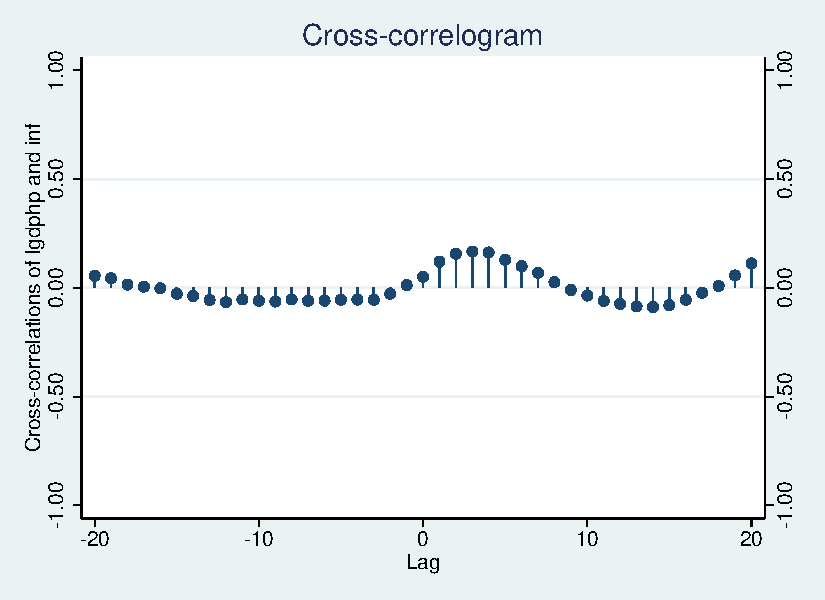
\includegraphics[width=7cm, height=7cm, keepaspectratio]{images/xcorr}
\caption{The output gap and inflation}
\end{figure}
{\footnotesize{The Figure shows a cross-correlogram between the output gap (estimated with a \textbf{two-side HP filter}) and inflation in South Africa. The cross-correlogram shows a mild effect of the output gap on subsequent inflation, but no evidence of inflation leading the output gap as would be required by an NKPC with this output gap. (Burger and du Plessis, 2006)}}
\end{frame}


\begin{frame}
\frametitle{Inflation inertia}
\begin{align*}
\mathbb{E}_{t}\pi_{t+1} - \pi_{t} = \underbrace{\frac{1-\beta}{\beta}}_\text{small$\approx$0.01} \pi_{t} - \frac{\kappa}{\beta}\underbrace{(y_{t} - \bar{y}_{t})}_\text{$\approx$ real MC}
\end{align*}
\small
\begin{itemize}
  \item Two shortcomings were revealed through empirical analysis
  \begin{enumerate}
  \item \textbf{Fuhrer and Moore} (1995)$\rightarrow$ output gap tends to lead inflation
  \begin{itemize}
    \item Sluggishness adjustment of prices observed in data
    \item Hump shape response to monetary policy (\textbf{not jump variable})
  \end{itemize}
  \item \textbf{Ball} (1994) $\rightarrow$ disinflation is costly, associated with recession
  \end{enumerate}
\item However, there is still some hope!
\item \textbf{Christiano, Eichenbaum and Evans} (2001) show that persistent effects are possible
\begin{itemize}
  \item They achieve this through introduction of habit formation, variable capital utilisation and investment adjustment costs
\end{itemize}
\item It might also be that our measure of the output gap is poor, rather use marginal cost?
\end{itemize}
\end{frame}


\begin{frame}
\frametitle{Perhaps labour share (MC) works better}
\begin{figure}
\centering
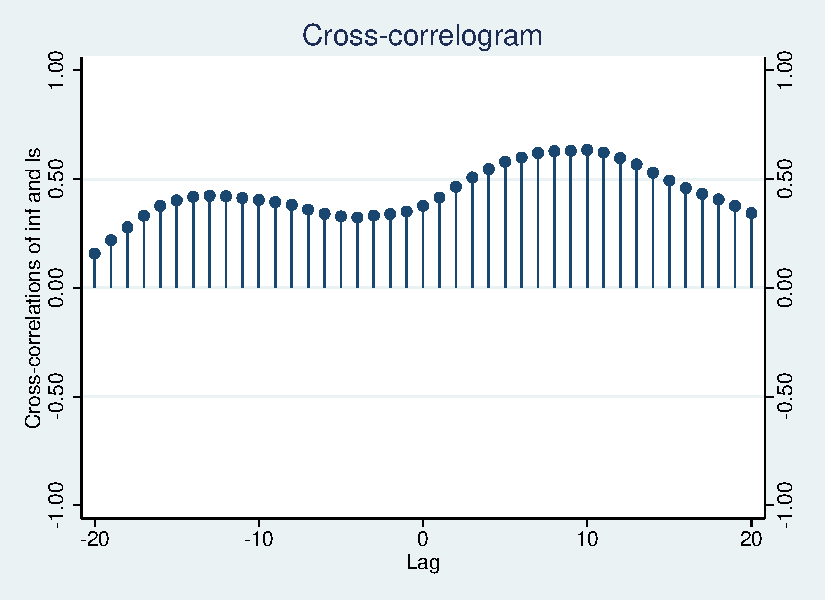
\includegraphics[width=7cm, height=7cm, keepaspectratio]{images/xcorr1}
\caption{Inflation and the labour income share}
\end{figure}
{\footnotesize{The cross-correlogram between the labour income share and inflation in South Africa shows that, empirically, inflation anticipates movements in the labour income share as required by the alternative specification of the NKPC. (Burger and du Plessis, 2006)}}
\end{frame}


\begin{frame}
\frametitle{Hybrid Phillips Curve}
\small
\begin{itemize}
  \item \textbf{Fuhrer} (1997) nests the traditional expectations augmented Phillips curve (\textcolor{blue}{accelerationist}) and the NKPC
  \item The model is also derived from microfoundations, and is given by,
\begin{align*}
\pi_{t} &= \kappa({y_{t} - \bar{y}_{t}}) + \gamma_{f}\mathbb{E}_{t}\pi_{t+1} + \gamma_{b}\pi_{t-1} \\~\\
\text{where} \quad\lambda &= \frac{(1-\omega)[1-\beta\theta][1-\theta ]}{\theta } \\
\gamma_{f} &= \frac{\beta\theta}{\phi} \\
\gamma_{b} &= \frac{\omega}{\phi} \\
\phi &= \theta + \omega[1-\theta(1-\beta)]
\end{align*}
\item Allows for a proportion of backward looking price setters $\omega$
\item Sometimes in the literature you will see $\theta = (1-\alpha)$
\end{itemize}
\end{frame}



\begin{frame}
\frametitle{Hybrid Phillips Curve}
\small
\begin{itemize}
\item \textbf{Gali and Gertler} (1999) take a formal econometric approach and try to estimate this equation, substituting output with marginal cost (and adding a disturbance term)
\begin{align*}
\pi_{t} = \lambda{S_{t}} + \gamma_{f}\mathbb{E}_{t}\pi_{t+1} + \gamma_{b}\pi_{t-1} + e_{t}
\end{align*}
\item Link between output and marginal cost $\rightarrow$ when output is above normal, marginal cost is high and relative prices are increased
\item They use labour share of income $S_{t}$ as proxy for marginal cost
\item However, \textbf{Rudd and Whelan} (2005) provide evidence against the usage of $S_{t}$ as a measure of marginal cost
\end{itemize}
\end{frame}


\begin{frame}
\frametitle{Alternatives to the NKPC}
\begin{itemize}
\item Hybrid NKPC (includes price indexing) $\rightarrow$ \textbf{Christiano, Eichenbaum and Evans}
\begin{itemize}
\item Not a single price, but rather past inflation indexed price path
\end{itemize}
\item Sticky information Phillips curve $\rightarrow$ \textbf{Mankiw and Reis} (2002)
\begin{itemize}
\item Rather than assume firms cannot adjust their prices, assume they infrequently update their information
\item Nominal rigidity $\rightarrow$ changes are based on \textbf{information not price}
\item Model predicts \textbf{inflation inertia} and no boon for announced disinflation
\end{itemize}
\item \textit{Generalized} New-Keynesian Phillips Curve $\rightarrow$ \textbf{Ascari and Sbordone} (2014)
	\begin{itemize}
	\item positive trend inflation: $\pi > 0$ in steady state
	\item standard NK models assume zero trend (steady state) inflation, such that: $\pi=0 \rightarrow i=r$ in steady state.
	\item implications: determinacy and stability region for monetary policy shrinks (requires more \textbf{hawkish} policy); generates endogenous \textbf{persistence} and real economic (\textbf{welfare}) costs via price dispersion; interacts with price indexation (\textbf{adaptive} expectations) and the elasticity of substitution (\textbf{markups})
	\end{itemize}
\end{itemize}
\end{frame}


\begin{frame}
\frametitle{South African Evidence}
\begin{itemize}
\item \href{https://www.resbank.co.za/content/dam/sarb/publications/conference-papers/2007/56/Du+Plessis.pdf}{\textbf{Burger and du Plessis}} (2006) look at several versions of the NK Phillips curve
\begin{itemize}
\item NKPC with labour income share merits consideration in the study of SA inflation dynamics
\item Parameter estimates are sensitive to model specification and sample periods, and often subject to weak instrument problems
\item Find that prices are fixed on average, for the sample period 1985Q1$-$2003Q4, between 3.5 and 4 quarters. 
\end{itemize}
\item \href{https://doi.org/10.1111/saje.12066}{\textbf{Reid and du Rand}} (2015) estimate a Sticky Information Phillips Curve {\'{a}} la Mankiw and Reis
\begin{itemize}
\item Find that the marginal cost calculation approach is not suited to the South African case
\item Prices are fixed for around 1.3 quarters
\end{itemize}
\item \href{https://doi.org/10.1111/saje.12192}{\textbf{Fedderke and Liu}} (2018) look at a range of inflation models: Phillips curve, New Keynesian Phillips curve, monetarist and structural models of inflation
\begin{itemize}
\item the single most robust covariate of inflation is unit labour cost, decomposed into the nominal wage (strong positive relationship) and real labour productivity (weak negative relationship).
\item  inflationary pressure: output gap does not statistically robust; money growth and govt. expenditure robust.
\end{itemize}
\end{itemize}
\end{frame}


\begin{frame}
\frametitle{South African Evidence}
\begin{itemize}
\item \href{https://www.resbank.co.za/content/dam/sarb/publications/working-papers/2020/WP\%202013.pdf}{\textbf{Viegi and Dadam}} (2020) estimate a New Keynesian Wage Phillips Curve $-$ wage formation mechanism very insensitive to overall macroeconomic conditions
\item  \href{https://ideas.repec.org/p/rbz/wpaper/10211.html}{\textbf{Botha, Kuhn, and Steenkamp}} (2020) consider an augmented Phillips curve specification that accounts for various drivers of inflation and test different measures of economic slack in forecasting inflation and GDP outcomes
\begin{itemize}
\item show that a Phillips curve relationship continues to exist in South Africa.
\item the slack measure that performs best is one that includes labour market indicators.
\item While the output gap-inflation channel continues to operate, the contributions to inflationary pressures of factors such as past inflation and inflation expectations have been much more important over recent years
\end{itemize}
\item \href{https://ideas.repec.org/p/unu/wpaper/wp-2023-79.html}{\textbf{du Rand, Hollander, and van Lill}} (2023) estimate the Phillips curve relationship using a novel deep learning technique.
\begin{itemize}
\item multiple measures of economic slack/tightness and inflation expectations
\item long-run inflation expectations are the dominant determinant of inflation, with these expectations anchored around 5\% historically but declining since the 2008 global financial crisis.
\item renewed empirical support for the relevance of the Phillips curve: short-run expectations and real economic activity are significant 
\end{itemize}
\end{itemize}
\end{frame}	


\begin{frame}
\frametitle{Hemisphere Neural Network Phillips Curve}
\begin{figure}
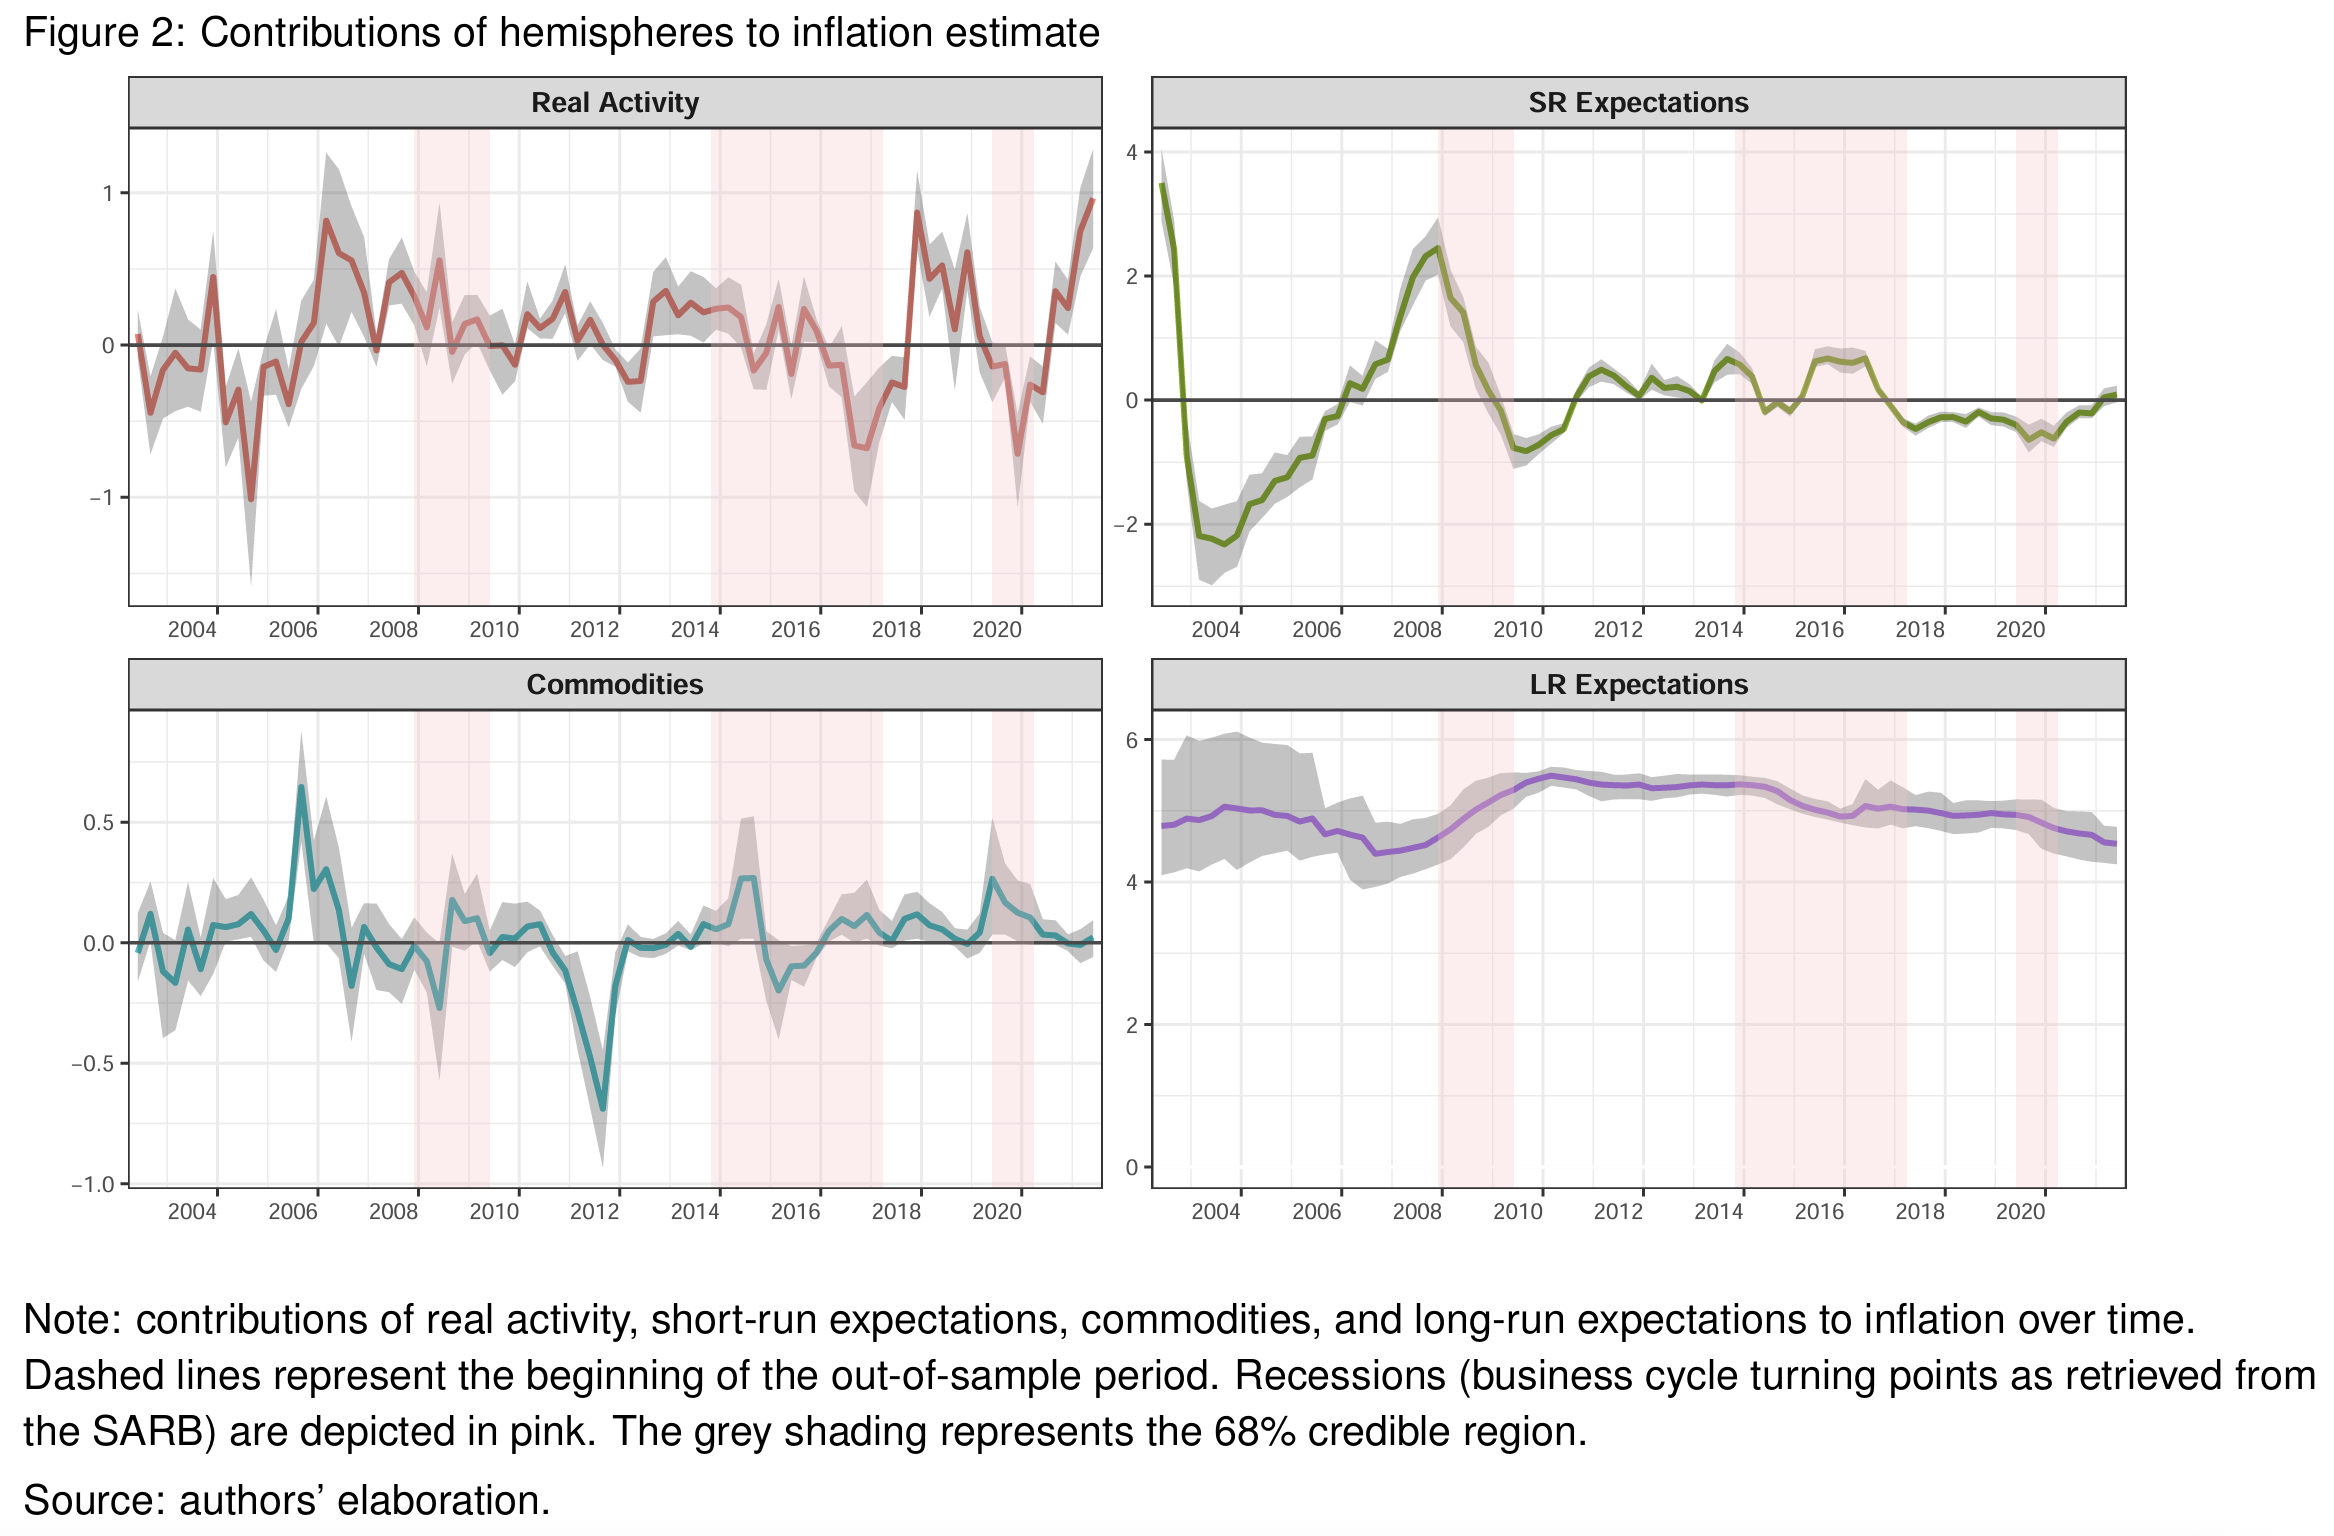
\includegraphics[width=0.85\textwidth]{images/dHv_2023_PCneural.png}
\caption{{\footnotesize{du Rand, Hollander, and van Lill (2023)}}}
\end{figure}

\end{frame}	


\begin{frame}\frametitle{The Canonical NK model}
The canonical three-equation new Keynesian model of Clarida, Gal{\'{i}}, and Gertler (2000)
\begin{itemize}
\item The price-adjustment equation is the new Keynesian Phillips curve of Section 7.4
	\begin{itemize}
	\item strong microeconomic foundations
	\item comparative simplicity
	\end{itemize}
\item The aggregate demand equation of the model is the new Keynesian IS curve of Sections 6.1 and 7.1.
\item The final equation describes monetary policy
	\begin{itemize}
	\item we assume the central bank follows \textit{a forward looking interest-rate rule}, adjusting the interest rate in response to changes in expected future inflation and output.
	\end{itemize}
\end{itemize}
\end{frame}

\begin{frame}\frametitle{The Canonical NK model}
The three core equations are:
\begin{eqnarray} \label{eq:nkis}
y_t &=& E_t\left[y_{t+1}\right]-\frac{1}{\theta} r_t+u_t^{IS}, \quad \theta>0, \\ \label{eq:nkpc}
\pi_t &=& \beta E_t\left[\pi_{t+1}\right]+\kappa y_t+u_t^\pi, \quad 0<\beta<1, \quad \kappa>0, \\ \label{eq:nktaylor}
r_t &=& \phi_\pi E_t\left[\pi_{t+1}\right]+\phi_y E_t\left[y_{t+1}\right]+u_t^{MP}, \quad \phi_\pi>0, \quad \phi_y \geq 0 .
\end{eqnarray}
Equation (\ref{eq:nkis}) is the new Keynesian IS curve, (\ref{eq:nkpc}) is the new Keynesian Phillips curve, and (\ref{eq:nktaylor}) is the forward-looking interest-rate rule. The shocks follow independent AR-1 processes:
\begin{eqnarray}
u_t^{IS} &=& \rho_{IS} u_{t-1}^{IS}+e_t^{IS}, \quad -1<\rho_{I S}<1, \\
u_t^\pi &=& \rho_\pi u_{t-1}^\pi+e_t^\pi, \quad -1<\rho_\pi<1, \\
u_t^{MP} &=& \rho_{MP} u_{t-1}^{MP}+e_t^{MP}, \quad -1<\rho_{M P}<1,
\end{eqnarray}
where $e^{IS}, e^\pi$, and $e^{MP}$ are white-noise disturbances that are uncorrelated with one another.
\end{frame}


\begin{frame}\frametitle{The Canonical NK model}

Next session we will do a practical application of the NK model. You can use any variation to compare to this baseline, for example:
\begin{itemize}
\item NKPC with indexation (simply replace the forward-looking NK equation with the equation (7.76) on p. 344, Section 7.7.
\item Alternative MP rules
\item Habit formation, Sticky wages, Credit market (for these extensions you'll use pre-existing code)
\end{itemize}
Discussion:
\begin{itemize}
\item The model's implications for the costs of disinflation (e.g., SARB moving from 4.5\% to 3\%)
\end{itemize}

\end{frame}


\end{document} 